


\documentclass[
%  handout
unknownkeysallowed
]{beamer}

\mode<presentation> {
\usetheme{strand}
}

%\usepackage{appendixnumberbeamer}


\usepackage{graphicx} % Allows including images
%\usepackage{colortbl}
\usepackage{physics}
%\usepackage{array}
\usepackage{transparent}
\usepackage{siunitx}
%\usepackage{tikz}

\usepackage[normalem]{ulem}
%\usepackage{cancel}

\graphicspath{{./Figures/},{./Images/},{./}}






\DeclareSIUnit{\au}{{a.u.}}



\let\thefootnote\relax
\renewcommand{\footnoterule}{%
  \kern -3pt
  \hfill\rule{0.65\textwidth}{0.005pt}
  \kern 2pt
  \vspace{1.5mm}
}




%%%% Title page
\title[Footer left]{Beamer theme: Strand}

\subtitle[Footer middle]{\ }

\titlegraphic{
\includegraphics[height=12.5mm]{KCL-Logo.png}}

\author{Emilio Pisanty}
\institute{\ }

\date{\today}

\begin{document}




{
\begin{frame}
\titlepage
\end{frame}
}




\begin{frame}
\frametitle{ }

This is a sample slide.

\begin{itemize}
\item
Bullet point

\pause
\item
Another bullet point
  \begin{itemize}
  \item Sub-bullet point
  \item Another sub-bullet point
  \end{itemize}

\pause
\item
A final bullet point

\end{itemize}

\end{frame}





\begin{frame}[fragile] %% the [fragile] should be removed -- it is there to protect the occurrence of \verb in this frame.
\frametitle{Figures and references}
Some text above a figure with a reference\\
\begin{center}
\only<1-2>{
  \only<1>{\transparent{0.2}}
  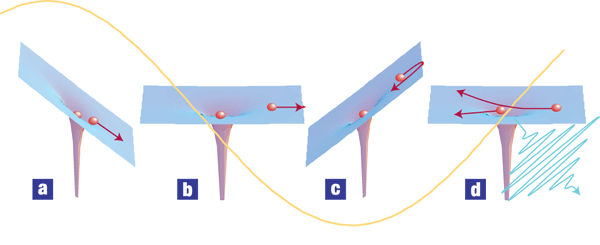
\includegraphics[width=0.85\textwidth]{CorkumFigure.png}
  }
\only<3>{
  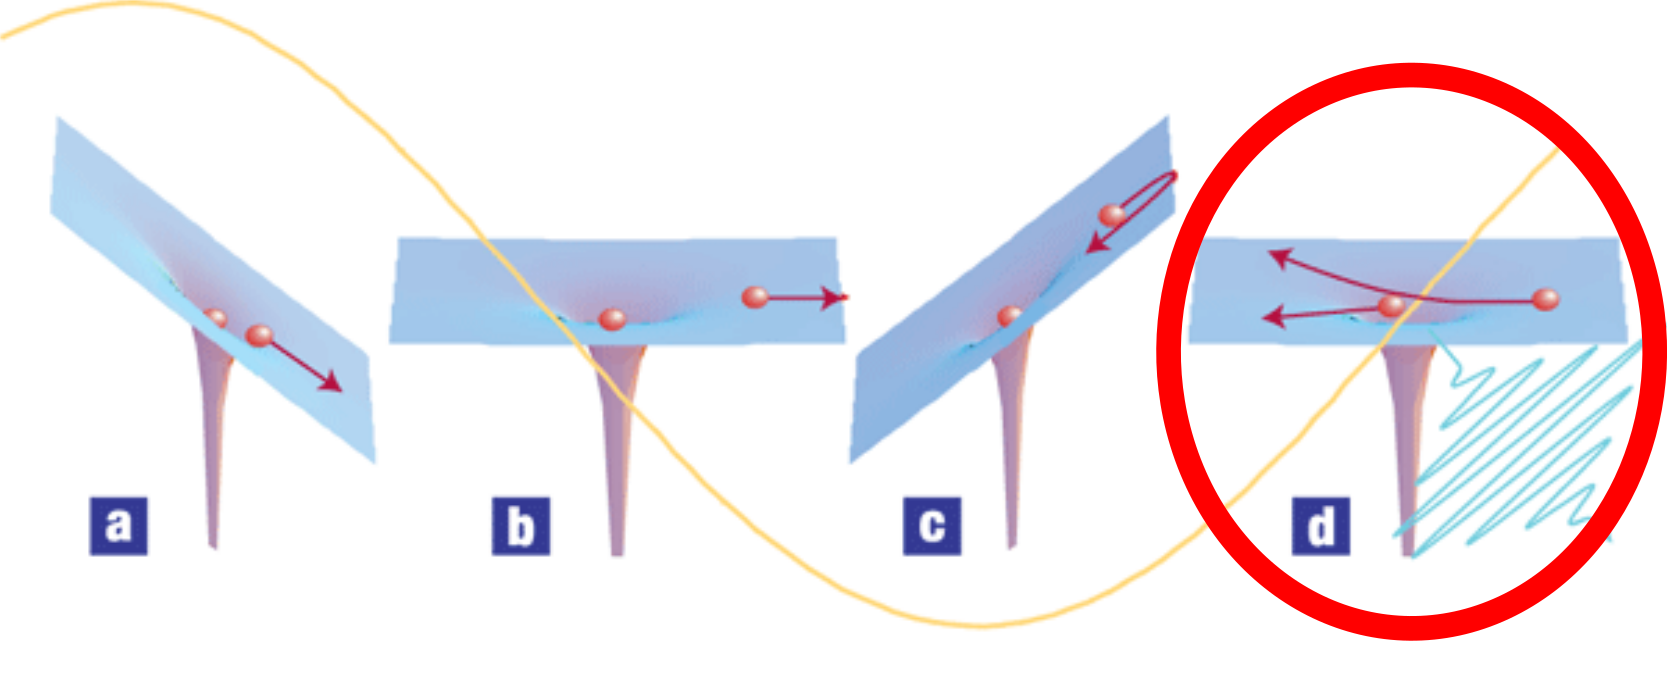
\includegraphics[width=0.85\textwidth]{CorkumFigure2.png}
  }
\vspace{-2mm}
\end{center}
The figure can be set to transparent and to change over the slides using the syntax \verb|\only<>{}|. This requires multiple compilations to converge to final form.
%
\footnotetext{
\hfill \scriptsize
Corkum \& Krausz, \textit{Nat Phys} \textbf{3}, 381 (2007)
\vspace{0.mm}}
\end{frame}





\newlength{\mugshotheight}
\setlength{\mugshotheight}{0.4\textheight}
\begin{frame}
\centering
{\huge Thank you!}

\vspace{15mm}

\tiny
\begin{tabular}{cccc}
%\includegraphics[height=\mugshotheight]{CollaboratorPhoto1.jpg}
%&
%\includegraphics[height=\mugshotheight]{CollaboratorPhoto2.jpg}
%&
%\includegraphics[height=\mugshotheight]{CollaboratorPhoto3.jpg}
%&
%\includegraphics[height=\mugshotheight]{CollaboratorPhoto4.jpg}
%\\
Collaborator 1
&
Collaborator 2
&
Collaborator 3
&
Collaborator 4
\\
Place 1
&
Place 2
&
Place 3
&
Place 4
\end{tabular}


\end{frame}










\end{document}
















